\chapter[Continuous Integration, Delivery \& Deployment]{\IfLanguageName{dutch}{Continuous integration, delivery \& deploy}{Continuous integration, delivery \& deployment}}
\label{ch:ci-cd-cd}
Bedrijven zijn constant op zoek naar betere en snellere resultaten, maar in de wereld van IT is het vandaag soms nog lang wachten voor een wijziging effectief wordt doorgevoerd. Vaak wordt een enorme hoeveelheid software op het einde van een sprint opgeleverd, stukken code van verschillende developers moet op het laatste nippertje nog aan elkaar worden geplakt om toch een werkende applicatie te bezorgen, wat soms problemen met zich meebrengt.\\
Met een vrij recente software development methode - Continuous Integration en Continuous Delivery genaamd - wil men hier verandering in brengen. Er wordt vaak gesproken van een CI/CD pipeline als het gaat over Continuous Integration en Continuous Delivery, maar er is nog een derde speler dat men kan invoeren: Continuous Deployment. Samen vormen zij de drie musketiers om software projecten een grotere slaagkans te geven.\\
Om een duidelijker beeld te scheppen van een CI/CD pipeline zal dit hoofdstuk eerst uitleg verschaffen over DevOps, omdat dit de allesomvattende term is waar de 3 musketiers deel van uitmaken. Er wordt ook dieper ingegaan op Continuous Integration, Continuous Delivery, Continuous Deployment en tot slot komt Automated Testing aan bod.
        \section{DevOps}
        DevOps is een samentrekking van development en operations en is een welbekend begrip binnen de informatica wereld. Het heeft als doel om de 'state of mind' binnen een bedrijf te veranderen zodat alle lagen/departementen vlotter samenwerken. Het is een praktische 'gids' die bedrijven kunnen hanteren om de communicatie tussen developers en systeembeheerders vlotter te laten verlopen. Deze twee verschillende lagen in een bedrijf willen namelijk hetzelfde: zo snel mogelijk, kwaliteitsvolle software opleveren. DevOps is gebaseerd op Agile development, maar gaat verder dan dat. Het gaat dieper in op automatisatie, integratie, samenwerking en communicatie. 
        Continuous Integration, Delivery en Deployment zijn kenmerkend voor DevOps, omdat het mee inzet op snellere oplevering van kwaliteitsvolle software. ~\autocite{Riti2018}
    
        \section{Continuous Integration}
        Dit is de eerste laag van de pipeline die zelf uit verschillende stappen bestaat. Eerst moet de geschreven code worden verstuurd naar een 'repository management server' aan de hand van een commit. De 'source code' wordt automatisch gebuild en bekeken of ze slaagt voor de automatisch gestarte testen. De focus bij deze stap ligt bij de teamleden ~\autocite{Fowler2006}, van hen wordt verwacht dat ze - op regelmatige basis - hun code pushen (integreren met de master applicatie). Een goede samenwerking tussen de verschillende leden van het development team is broodnodig om tot het gewenste eindresultaat te komen.
        Het doel van een Continuous Integration is om de integratie feilloos te doen verlopen wanneer men software ontwikkelt en geen functionaliteiten verliest na een merge ~\autocite{Riti2018}.
        
        Bovenstaande uitleg is makkelijker te begrijpen aan de hand van een voorbeeld. Op Figuur \ref{img-ci-example} is een grafische voorstelling van onderstaande uitleg terug te vinden.
        De developer maakt een wijziging en commit de code naar de repository, die te vinden is op het source-control systeem, zie \ref{subsec:source-control-systeem} voor verdere uitleg. De Continuous Integration server (CI server) krijgt bericht dat er code is toegevoegd, haalt de laatst toegevoegde code op en laat de geschreven unit testen runnen. Wanneer alle testen slagen zal de CI server de code compilen en feedback bezorgen aan de developer. In dit voorbeeld is er gebruik gemaakt van een externe mail server om die feedback te verzenden.
        Deze stappen gebeuren telkens er nieuwe code naar de repository wordt gestuurd.
        
        De uitleg die hierboven te lezen valt, is een best-practice hoe het zou moeten gebeuren. Hieronder worden een aantal zaken extra toegelicht.
        De frequentie en hoeveelheid code zijn belangrijke zaken waar de developer rekening mee moet houden bij een CI pipeline. Volgens \textcite{Fowler2006} is het de plicht van een developer om minstens één maal per dag een commit uit te voeren, telkens wanneer hij een kleine opdracht afgerond heeft. Zo blijft de hoeveelheid code klein en is het makkelijk om te zoeken wanneer er zich een probleem voordoet.
        Eens de wijziging gecommit is naar de version control repository moet de CI pipeline zijn werk doen. Een belangrijke stap is het bezorgen van feedback. Dit moet bestaan uit het resultaat van de build en de beschrijving van het probleem, alsook de plaats waar het probleem zich voordoet, door bijvoorbeeld aan te geven welke test niet slaagt. De belangrijkste factor hier is tijd. Als de developer pas daags nadien feedback krijgt over de fout die hij gepusht heeft, wordt het al moeilijker om de fout te vinden en ze op te lossen. 
        \begin{figure}	
            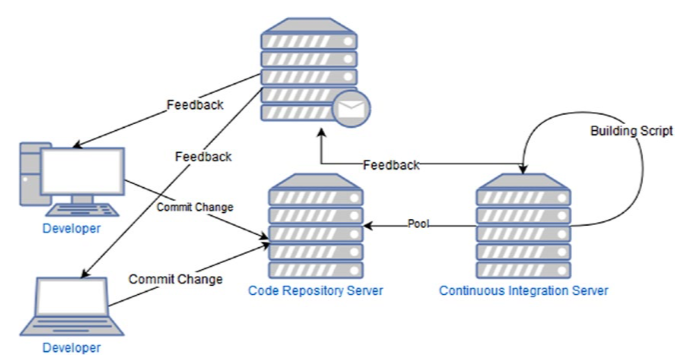
\includegraphics[scale=0.65]{ci-example}
            \caption{Voorbeeld van een Continuous Integration set-up ~\autocite{Riti2018}} \label{img-ci-example}
        \end{figure}
    
        \section{Continuous Delivery}
        Eens het team met succes de Continuous Integration toepast kan men overschakelen naar de volgende stap: Continuous Delivery.
        Het is een manier die ervoor zorgt dat de code die van de Continuous Integration stap komt, wordt gebuild en voorbereid voor een release.
        Er is echter wel nog een menselijke hand nodig om de build van deze stap te deployen en voor de buitenwereld beschikbaar te stellen ~\autocite{Fowler2013}.
        \newline{}In Figuur \ref{img-cd-chain} wordt de opbouw van een Continuous Delivery chain weergegeven, het is een grafische weergave van de stappen waaruit een Continuous Delivery pipeline moet bestaan. Dit is gebaseerd op de Continuous Integration chain, maar hier zijn extra stappen toegevoegd.
        
        De eerste stap is het developen van de code die men wenst op te leveren. Net zoals bij Continuous Integration commit de developer de code naar de version control repository. De build scheduler haalt de laatst toegevoegde code op en test deze code. Enkel bij het slagen van alle testen wordt de code gebuild door de build scheduler en nog verder door de testmolen gehaald. Hier worden de integratietesten uitgevoerd en wordt gekeken of de code voldoet aan de kwaliteitseisen van een release. Eens de build slaagt voor alle testen wordt deze door de build scheduler klaar gemaakt voor release. Het vereist enkel nog menselijke goedkeuring om deze release te lanceren.
        \newline{}In dit proces is feedback ook uiterst belangrijk. Wanneer developers foute code pushen, moet de persoon die de foute code heeft geschreven zo snel mogelijk worden verwittigd. Op deze manier kan het euvel snel worden opgelost en kan er niet verder worden gebouwd op foutieve code.
        Mail kan een vorm zijn van feedback, maar er bestaan nog andere leuke vormen naast mailing.\\
        Het bedrijf Dynatrace heeft bijvoorbeeld een licht ontworpen dat je in de kamer van het team kan hangen. Dit Internet of Things (IoT) gadget, DevOps UFO genaamd, is via WiFi verbonden met de pipeline omgeving. Het geeft rechtstreekse feedback over de staat van de CI/CD pipeline en is een vorm van monitoring. Als de commit door de pipeline geraakt zal de UFO groen kleuren, wanneer de build faalt kleurt de UFO rood en weet iedereen dat er een fout naar de CI server is gebracht. Zo weet de persoon die de foute code heeft gepusht dat er iets fout is en kan hij hier nog sneller op inspelen. 
        \begin{figure}	
            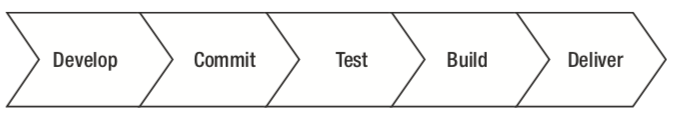
\includegraphics[scale=0.65]{cd-chain}
            \caption{Continuous Delivery chain ~\autocite{Riti2018}} \label{img-cd-chain}
        \end{figure}
        
        \section{Continuous Deployment}
        De gelijkenis met Continuous Deployment is treffend, maar er is wel degelijk een verschil.
        Hier gaat men automatisch de veranderde code naar productie brengen. De veranderingen gaan door de volledige pipeline en eens ze slagen voor alle testen wordt - zonder menselijke interactie - de code naar productie gebracht ~\autocite{Claps2015}.
        Dit wordt soms ook wel de 'train to production' genoemd, omdat elke code dat wordt gepusht naar de source-control automatisch tot bij de klant geraakt.
        
        \section{Automated Testing}
        Zoals hierboven reeds is aangegeven, is er geen Continuous Integration pipeline zonder automated testing. Het grootste doel van deze fase is - zoals de naam het zegt - testen van de code. Als de CI/CD pipeline wordt voorzien van voldoende en goede testen, creëert dit een veiligheidsgevoel. Op deze manier voldoet de software aan bepaalde criteria, die in de testen worden verwerkt. Het is dus een heel belangrijk onderdeel van de pipeline waar veel aandacht aan besteed moet worden. 
        Om te voldoen aan de criteria van CI/CD moeten de testen automatisch worden gerund. Dit was tot voor kort echter vaak niet het geval. Er werden testers aangesteld om telkens opnieuw software te testen, door op de verschillende knoppen te drukken in de user interface (UI). Heel vaak slopen er fouten in omdat dit heel repetitief en saai werk was. Daar komt de automatisatie van pas ~\autocite{Vocke2018}.
        
        Mike Cohn kwam met het idee om testen op te delen in drie grote categorieën: Unit Tests, Service Tests en UI tests zoals u kan zien in figuur \ref{img-test-pyramid}.
        Twee zaken zijn belangrijk om te onthouden: testen moeten uit verschillende lagen van detail bestaan en er moeten minder testen worden geschreven wanneer het team minder gedetailleerde code schrijft (high-level testing). Omdat bij high-level testen de requirements goed begrepen zijn door het test team.
        
        De grootste laag binnen de test omgeving zijn de Unit tests en staat het dichts bij de software code. Deze testen zijn snel om te schrijven en te runnen en kunnen gedetailleerde feedback geven wanneer een test faalt.\\
        De laag erboven zijn de service tests - ook wel Integration tests genoemd - en focussen vooral op de functionaliteit van de applicatie. Ze testen de API calls en de integratie van de individuele functies.\\
        De kleinste laag zijn de UI tests, ook wel end-to-end testen genoemd. Deze testen de user interface door bijvoorbeeld op knoppen te drukken, formulieren in te vullen of te navigeren doorheen de applicatie. Het nadeel van deze testen zijn dat ze fragiel, duur en tijdrovend zijn om te bouwen en traag om te runnen.
        Om de snelheid te garanderen en de hoeveelheid build times klein te houden is het belangrijk de vorm van de piramide te behouden. Het gevaar dreigt om de test omgeving als een ijsjeshoorn te vormen met meer UI tests dan Unit tests ~\autocite{Fowler2012}.
        \begin{figure}
            \centering
            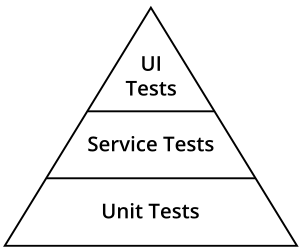
\includegraphics[scale=0.65]{test-pyramid}
            \caption{Test piramide ~\autocite{Vocke2018}} \label{img-test-pyramid}
        \end{figure}
        
        Vandaag zijn deze categorieën iets te simplistisch voorgesteld, vanwege de toenemende complexiteit van de software. Maar het is wel nog altijd een uitstekende referentie om de opbouw van testen uit te leggen.
        De Automated Test Quadrant is een voorbeeld waarop een test omgeving kan worden gebaseerd, zoals in figuur \ref{img-test-quadrant} te zien is. Het is ook model, net zoals de test piramide en is bedoeld als gids. Er bestaan verschillende modellen waarop je je kan baseren.
        
        De Automated Test Quadrant deelt de testen op in vier categorieën op basis van hun rol en complexiteit.\\
        De eerste kwadrant focust op de logica aan de business-zijde en zijn high-level (bevatten weinig details). De tweede testen veel details die te maken hebben met de business logica die de klant wenst.\\
        De derde kwadrant zijn testen die zijn geschreven met de toekomst in het achterhoofd. Ze testen of de applicatie makkelijk uitbreidbaar is. De vierde soort test de technische zaken zoals het gebruik van de API enzovoort ~\autocite{Smart2017}.
        
        \begin{figure}
            \centering
            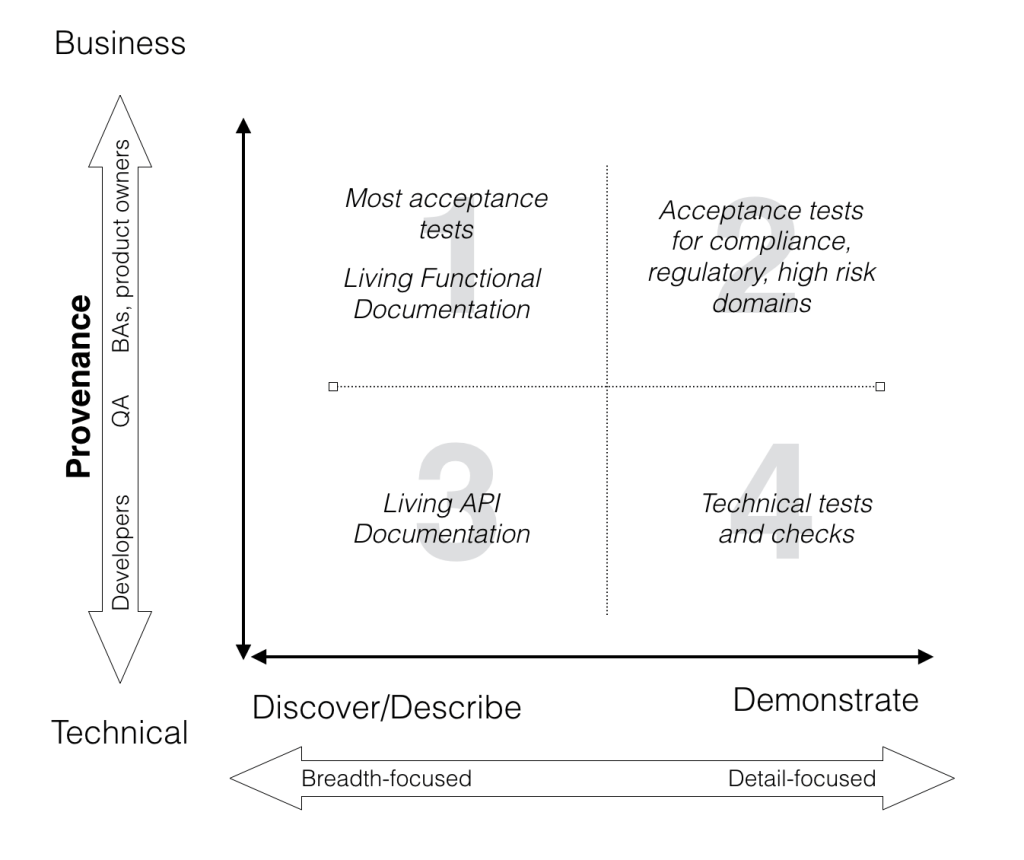
\includegraphics[scale=0.65]{test-quadrant}
            \caption{Automated Test Quadrant ~\autocite{Smart2017}} \label{img-test-quadrant}
        \end{figure}